%%%%%%%%%%%%%%%%%%%%%%%%%%%%%%%%%%%%%%%%%%%%%%%%%%%%%%%%%%%%%%%%%%% 
%                                                                 %
%                            CHAPTER SEVEN                        %
%                                                                 %
%%%%%%%%%%%%%%%%%%%%%%%%%%%%%%%%%%%%%%%%%%%%%%%%%%%%%%%%%%%%%%%%%%% 
 
\chapter{CONCLUSION AND FUTURE WORK}
Semantic importance (SI) provides a flexible way to model the importance of the streaming data from various data orderings.
The evaluation results have partially shown evidence that SI is capable of reducing system overhead and increasing system performance. 
The flexibility lies in the fact that SI supports a range of window management strategies that can efficiently manage the data in the window. 
In this thesis, I have instantiated the SI ontology by providing an extensive soccer offside example, thus showing how the SI ontology can be used in practice.
The SI ontology is implemented in OWL and can easily be browsed and extended using any of a number of open source ontology editing, browsing, and reasoning tools.
This chapter concludes this dissertation, and provides future insights on where SI can go from current standing point. 
%
\section{Conclusion}

\begin{figure}[!htbp]
	\centering
    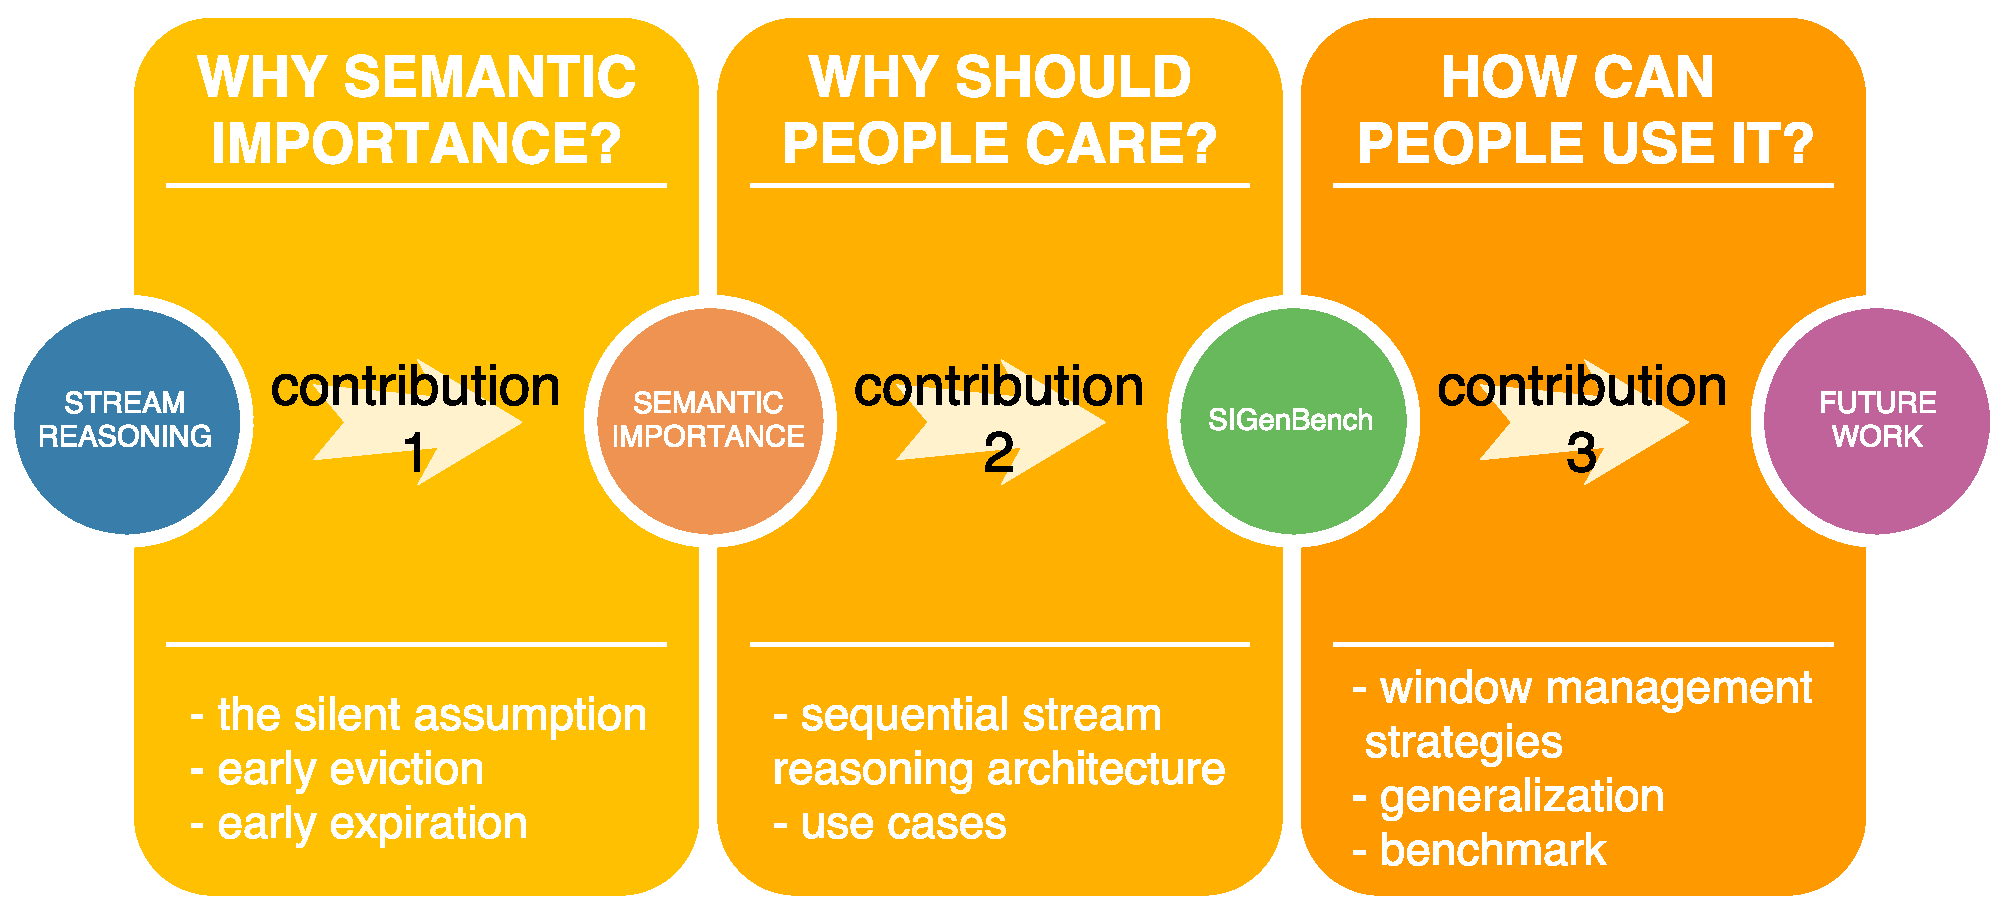
\includegraphics[width=5in]{img/7-trm.pdf}
    \caption{Thesis Road Map Overview}
    \label{fig:7-trm}
\end{figure}
%
\subsection{Thesis Brief Review}
Figure \ref{fig:7-trm} shows the road map overview of this thesis, which is generally guided by these three questions: 
``why semantic importance'', ``why should people care'', and ``how can people use it?''。
This thesis has rooted itself deeply into the stream reasoning, and targets on smart and flexible streaming data management. 

Chapter 3 covers my first contribution, semantic importance, which is motivated by the observations that the ``silent temporal assumption'' is popular across lots of stream reasoning research work \cite{barbieri2010stream}, \cite{stuckenschmidt2010towards}, \cite{golab2003processing}, \cite{barbieri2010deductive}, and that temporality alone will not work under the situations where the early eviction or expiration problem happens. 
Semantic importance models the data importance by considering aspects beyond just temporality, such as query participation, query relevance and trustworthiness. 
It provides a representative schema (using the priority vector technique), as well as a set of defined comparison rules to enable data orderings. 
This answers the first question, ``why semantic importance''.

Chapter 4 introduces the sequential stream reasoning architecture (SSRA). 
It is motivated by the fact that stream reasoning engines such as C-sparql and CQELS are implemented using the silent temporal assumption, and do not provide an interface to deploy the semantic importance. 
I have implemented and evaluated SSRA comprehensively.
Basically I have classified three streaming scenarios and analyzed some semantic importance enabled strategies' performance. 
In order to ground both semantic importance and SSRA, I have described my implementation of two use cases in Chapter 5, namely soccer offside detection and data exfiltration detection.
This thesis has covered detailed implementations and evaluations, and the results show that semantic importance can work under fairly diverse scenarios, as well as provide good precision and response time. 
However, the use cases described have some limitations, which I have investigated and explained in this thesis. 
Thus, the answer to the second question is that, people should care about semantic importance because it can work better than the most commonly used strategies (e.g., FIFO) in the cases where temporality alone is not enough
It can provide better system performance as well. 

Chapter 6 covers the work to generalize and benchmark semantic importance (SIGenBench).
Albeit the use case results have indicated that semantic importance is useful, it is not generalized so that a wide range of stream reasoning applications can use it in an easy way.
SIGenBench connects semantic importance to the state-of-the-art stream reasoning technologies.
It also comes with a default streaming data generator that simulates different streaming data scenarios. 
Extensive experiments have been done, and results have been analyzed. 
SIGenBench answers how people can use semantic importance.
%
\subsection{Thesis Wrap-up}

Starting from the Chapter 1, I have been using a running example of the soccer offside detection.
The purpose of this example is to illustrate the two problems of the streaming data management, i.e. early eviction and early expiration, if temporality is only considered to manage the data.

A window in a stream reasoning application will always evict the oldest data item in order to consume the latest data item, based on the silent temporal assumption, which means that the data is managed by its arrival timestamps: the older it is, the less important it is, thus it is evicted eventually. 
However, temporality is certainly not the only criterion to determine the data importance . 
In the running example, where players' status and positions are so important for the result, the ``who'' (who is
the attacker or defender?) and ``where'' (where are the players, onside or offside position?) provenance aspects should definitely be considered to manage the data. 
Thus, my first contribution -- semantic importance is able to provide a multi-dimensional view of the data importance and enable order-aware window management strategies, so that the important data can be captured.
Examples of the important data include but not limited to: Player A is an attacker, Player A is at an offside position, Player A touches the ball after his teammate passed the ball, etc. 
Please note that this important data usually does not arrive adjacently, in fact there could be lots of other data arriving in between.
By keeping the important data, semantic importance can be used to maintain a smaller window size, ideally only to contain the important data items for question-answering, which saves memory and response time.
Table \ref{tb:accuracy} has already shown that semantic importance enabled strategies (*-LFU-FO, *-LRU-FO, and QR-*) are able to maintain better precision and relatively lower response time than common strategy FIFO, even if the window size shrinks.
This has already shown the benefits of introducing semantic importance into stream reasoning, and how semantic importance can make the soccer offside offence detection better.

Instead of using a C-sparql or CQELS engine to implement the soccer use case, I used my sequential stream reasoning architecture (SSRA).
This is because I needed to enhance streaming data management with semantic importance, which is not supported in C-sparql or CQELS. 
SSRA is an example of deploying semantic importance in stream reasoning use cases. 
Its implementation imitates the behavior of other stream reasoning engines.
The soccer offside detection use case is implemented based on SSRA, and Table \ref{tab:ev} shows all the experimental results.
SSRA, as my second contribution, shows how semantic importance can be integrated, and performant in real life scenarios. 

My third contribution, SIGenBench, essentially targets a more general application, including but not limited to the soccer offside detection. 
The goal is to enable a broad view for semantic importance in the stream reasoning settings. 
The results from the soccer offside use case have already proven that semantic importance can work well. 
However, more questions need to be addressed, such as how to allow others to leverage semantic importance in their use cases, how to use the mainstream stream reasoning technologies with semantic importance, and under what conditions semantic importance can bring benefits. 
The answers to these questions are provided by SIGenBench. 
I have tested four aspects of the current semantic importance, and the results are provided in Table \ref{tab:6-qrp} - \ref{tab:6-fqqi} (query relevance), Table \ref{tab:6-dei} (temporal provenance), Table \ref{tab:6-qpp} (query participation), and Table \ref{tab:6-tp} (trustworthiness). 
SIGenBench comes with a default streaming data generator that can simulate different streaming data scenarios by configuring parameters such as stream mode and rate. 
The experiments indicate that trustworthiness and query relevance are both able to tolerate the large and fluctuating data streaming rate, yet query relevance does drop its performance when reaching a relatively large data rate. 
However, a compound strategy composed by multiple semantic importance aspects such as QR-Trust-FE-LFU-FI-FO is able to provide good performance.
%
\subsection{Thesis Key Takeaway Message}
The key message to take away is that, this thesis raises the awareness of the silent temporal assumption, and identifies some of the problems associated with temporality alone.
In order to loosen this assumption, this thesis provides a structure -- semantic importance, as well as a set of infrastructure components -- SSRA and SIGenBench to use this structure. 
The experimental results have shown that the smart and flexible window management can be enabled by modeling streaming data importance using semantic importance, as well as that the stream reasoning systems' precision, response time, memory consumption and throughput can be improved.
%
\subsection{Thesis Limitations}
Considering that streaming data is huge and can potentially flood the system, the sequential way to process the data clearly has a limit. 
Parallel processing has lots of benefits, one of them is to boost response time, there are already some examples to leverage distributed systems in stream reasoning \cite{hoeksema2011high}, \cite{liu2014efficient}. 

This thesis only deals with RDF streams, which is only a kind of all the streaming data.
However, in the traffic surveillance scenario, the streaming data is usually video format. 
This thesis doesn't propose a method for it. 

The query relevance is able to provide good response time and precision, however, as the data rate goes up from Figure \ref{fig:6-csmrrt1} - \ref{fig:6-csmrrt9}, query relevance spends much more time filtering the data and eventually causes a delayed answer. 
This is a major limitation for query relevance while being used in the sequential processing. 
However, I believe that a parallel infrastructure approach can diminish, if not eliminate, this limitation in many settings.
%
\section{Future Work}
This thesis has covered three contributions for managing the streaming data in the window for stream reasoning applications.
There is still lots of potential to extend and enhance this work. 
This section highlights some future work.
%
\subsection{Short Term}
This thesis has focused on the temporal provenance, albeit according to \cite{ram2009new}, there are six more aspects including ``what, where, how, who, which, and why''.
The soccer offside has leveraged where and who provenance, thus this thesis has shown some examples to extend different types of provenance.
I would like to extend the other aspects of provenance because they provide a broader view and more flexible way to model data importance.

Query relevance is an interesting aspect of semantic importance.
The experimental results have indicated its effectiveness. 
For the short term future work, I would like to investigate the general principles to prepare both the query relevance ontology and query relevance filter query. 
SIGenBench has shown that different query relevance filter queries do have different affects on system performance. 
If such general principles for preparing query relevance are proposed, the stream reasoning system as well as its users can benefit.
%
\subsection{Middle Term}
SIGenBench is built upon SSRA, which is sequential.
In the future, I would like to explore a parallel architecture approach and enhance it with distributed processing systems.

SIGenBench is implemented in Java, which is a static typed language.
All the 26 strategies are implemented as Java classes and hard-coded in the code. 
If a user wants to use a new strategy, he/she has to dive into my code and add a strategy class manually. 
There are two planned future lines of work to improve this. 
First of all, I would like to re-implement SIGenBench by exploiting a dynamic typed language, so that different strategy classes can be generated during run-time. 
Secondly, I want to build an ontology loader that can load the semantic importance ontology.
By combining semantic importance aspect classes, different strategies will be generated proactively. 
In that way, the semantic importance ontology will no longer be a merely descriptive ontology, but actually be used to create strategies.

Long short-term memory (LSTM) \cite{DBLP:journals/neco/HochreiterS97} is a recurrent neural network (RNN), whose cells can ``remember'' values over arbitrary time intervals \cite{lstmwiki}.
LSTM is potentially another way to implement window management strategy, which essentially can capture data items that are arbitrary apart, to alleviate early eviction problem. 
This is because how much data needs to keep is a similar requirement. 
I also would like to explore the possibilities to employ LSTM for the streaming data management. 

The default streaming data generator produces fluctuating data based on the observations of the traffic. 
The future work also includes simulating data bursts based on common burst patterns in other streaming data feeds such as smart city settings \cite{tonjes2014real}.

As we can see from the results in SIGenBench, when data rates increase, some previously working strategies start to fail.
This can also be found when the data fluctuates a lot.
I would like to investigate the possibilities to automatically switch strategies in the window so that the data management can be more resilient in different streaming scenarios. 
%
\subsection{Long Term}
In this thesis, with only 4 semantic importance aspects, I have created 26 strategies.
It can be predicted that as the semantic importance ontology is extended, more aspects will create more strategies. 
Certainly not all of the strategies will be useful or needed to implement the use case. 
I would like to build a strategy selector in the long time run, with which the users can easily select their desired strategies. 
In order to realize this, I need to collect data on users' use cases requirements and different strategies performance, which can be done with SIGenBench.
Then I will use supervised machine learning algorithms to train a model that can recommend strategies for users give their new use case requirements. 
This future work is dependent upon the general use of semantic importance. 
% \section{Conclusion}
% The core contribution of this dissertation is the notion of semantic importance, along with a set of infrastructure to enable its usage in the stream reasoning settings.
% Exemplar use case implementations have shown show how semantic importance can be leveraged in real-world scenarios.
% The comprehensive generalization and benchmark framework connects semantic importance to the state-of-the-art stream reasoning techniques, which allows testing system performances with multiple dimensional configuration parameters.

% The motivation to propose semantic importance originally comes from the situations where the temporal silent assumption can fail.
% The temporal silent assumption, which regards the most recent data as the most important, only concentrates on one explicit data ordering -- arrival order. 
% This will cause two problems, early eviction and early expiration, as it has been shown in Chapter 1.
% It has been observed that these two problems are caused because the system is not able to distinguish the data based on its priority. 
% Such priority, often implicit, leads to the efforts to make it visible for the processing system, which is formalized in the concept of semantic importance.
% Semantic importance is derived from various data orderings, and currently provides four general aspects that can support a wide range of window management strategies.
% Like FIFO, these strategies help window to identify more important data with one or multiple data orderings; but unlike FIFO, these strategies provide more flexible options to choose under different stream reasoning scenarios, which can improve system performance.

% Chapter 3 shows what semantic importance is, as well as its incompatibility with the existing window semantics that only works with FIFO.
% In order to deploy semantic importance in stream reasoning systems without breaking the integrity of window semantics, the landmark window is leveraged.

% The semantics of landmark window provide a firm theoretical foundation for the application of semantic importance. 
% Stream reasoning not only requires real-time stream processing, but also on-line reasoning.
% Most state-of-the-art work in stream reasoning performs logical reasoning, i.e., to provide a background ontology that contains the knowledge about the domain in the window.
% A reasoner also resides in the window, which can be used to infer hidden information together with the ontology and the streaming data. 
% However, logical reasoning is relatively slow, and does not scale well with large volume of data. 
% One method to minimize this problem is to reduce the data items in the window. 
% This can be done by either shrinking the window size or filtering the data. 
% When shrinking the window size, data items get more easily to exit the window under the silent assumption, but when filtering data, the system has to make sure to filter data correctly so that all the necessary data items are kept. 
% Both of them require the system to be data discriminative, which is enabled by semantic importance. 

% Semantic importance currently includes four aspects, provenance, query participation, trustworthiness, and query relevance. 
% It is designed to be flexible and extendable. 
% It also comes along with an ontology that is grounded by real-life use case and instances.
% Semantic importance is embodied in a priority vector, which features a preference function that the most preferred element is placed leftist, as well as a comparison rule that enables ranking.

% The semantics of sliding window, which works well with the temporal silent assumption, cannot be adopted when using semantic importance. 
% This is because, other than FIFO, the strategies enabled by semantic importance will evict the data out of its arrival order.
% This can break the semantics of the sliding window.
% Thus, the landmark window is proposed to use, as its semantics works well under the semantic importance framework. 
% Both time-based and tuple-based window semantics have been refined, which is not only compatible with the sliding window, but also opens up more window options to use in stream reasoning. 

% Chapter 4 introduces the sequential stream reasoning architecture (SSRA), with the purpose of providing the first architecture to deploy semantic importance for stream reasoning use cases. 
% SSRA features five main component, other than the window implemented in off-the-shelf triple-stores, the data consumption component consumes the data by sending it into the window. 
% Depending on different window report policies, the query execution component is fired and thus query results are generated. 
% The reasoner inside of the triple-store can provide the ability to trace back to what happened during the reasoning and query process, such that the data items participated in the query can be tracked.
% At last, the data is evicted based on its semantic importance ranking.
% Usually, the lower-ranked data will be evicted first. 

% SSRA shows how semantic importance can be deployed in a stream reasoning application, with experimental evidence that shows SI efficacy. 
% Since most state-of-the-art stream reasoning work is dependent on solely sliding window, which encapsulates the window and window strategies within the internal core, it is not feasible to implement semantic importance on the top of them. 
% However, their architecture and design can be referenced, which leads to the sequential stream reasoning architecture. 
% The core design is to let the window stand out of the processing architecture, so that it can be configured according to the users' need. 


% Chapter 5 shows two use cases implementations based on different window management strategies.
% Both of them are within the streaming context, where the data is either streamed in high frequency or large volume. 
% They are real-world use cases with different requirements.
% The results have shown that semantic importance is adaptable in different cases, and provide satisfactory system performance. 

% Chapter 6 generalizes semantic importance by connecting it to the state-of-the-art stream reasoning techniques, as well as provides a software that can benchmark the performance of stream reasoning applications.
% The experimental results have provided a systematical analysis on how different factors can affect the system performance, as well as how semantic importance can help minimize the adverse impacts and maximize the benefits. 
% SIGenBench is carefully implemented to decouple the window semantics out of its processing engine, such as C-sparql and CQELS. 
% Currently, SIGenBench supports four kinds of window, four kinds of window report operational semantics, two kinds of continuous query language, and twenty-four different window management strategies. 
% All of these open up a greater possibility to configure windows in many different ways. 
% SIGenBench can also control stream rates and modes, so as to provide more simulation capabilities. 
%
% \section{Future Work}
% Semantic importance currently only has four aspects, among which the provenance and trustworthiness aspects are both very broad. 
% This dissertation only talks about some temporal provenance, and leaves other types of provenance untouched. 
% For example, geographical location is an example of non-temporal provenance, and surely can be useful for some queries that involve geology.
% Query relevance is a very interesting aspect. 
% There are several ways to make it more interesting in the future.
% For example, formalize the general principles of preparing the query relevance ontology, although in Section 3.4 I have briefly mentioned this. 
% Since query relevance ontology is static and will only work with one query. 
% This hinders system if a different query is deployed. 
% Another direction is to come with a method to enable query relevance self-evolving ontology.
% Basically it can learn what is going on in the current stream and summarize some potential interesting knowledge. 
% From the experiments, it has also shown that different query relevance filtering queries have different impacts on system performances. 
% The next step also includes how to come up with good filter queries that maximize the performance gain, to formalize the criterion for categorizing and recognizing good, OK or bad queries.
% One future work is to explore and expand semantic importance both horizontally and vertically.

% SIGenBench is a tool that helps test semantic importance.
% It is configured with parameters in the command lines. 
% Users can feed their data, ontology, and choose their desired window and stream configurations before any experiments can run, from which the benchmark results will be generated.
% One restriction in this tool is that, all the strategies are currently built-in, which does not enable the user to choose their own desired strategies that are not listed within. 
% The reason is because SIGenBench is implemented in Java, which is a static type language, and does not support explicitly creating undeclared classes during the run-time. 
% There is really no solution to this in Java, thus what I did was to hard code all 26 strategies in the explicit class files and call them during the run time.
% There are two directions in the future work to enhance it.
% First, to implement SIGenBench in a dynamic typed language, so that the strategies can be created during the run-time.
% Second, the strategies will be supported by loading the semantic importance ontology, where the users extend, specify and edit their extended aspects.
% SIGenBench should be able to create a list of possible strategies on the top of reading semantic importance ontology and let the user to specify what strategy they would like to test in their use cases. 

% The third future work is a more ambitious one.
% As time goes by, during which semantic importance is being used and extended, as well as different use cases are being developed, the data of both use case requirements, the chosen management strategies and semantic importance aspects will become more and more available quantitatively and in quality.
% By leveraging such data and supervised machine learning algorithms, a recommendation system should be feasible to implement, and able to provide some constructive suggestions on which semantic importance aspects and strategies to use for new users, based on the input of their use cases. 
% The recommended results will be at least as a starting point from which the users will need to test their use case. 


 
% \chapter{CONCLUSION AND FUTURE WORK}
% Semantic importance (SI) provides a flexible way to model the importance of the streaming data from various data orderings.
% The evaluation results have partially shown that SI is capable of reducing system overhead and increasing system performance. 
% The flexibility lies in the fact that SI supports a range of window management strategies that can efficiently manage the data in the window. 
% SI is also expendable thanks to the SI ontology, which helps understand SI with grounding instances. 
% Implemented in OWL, SI ontology can be easily edited in ontology composing tools so that new aspects can be added. 
% This chapter concludes this dissertation, and provides future insights on where SI can go from current standing point. 
% %
% \section{Conclusion}

% \begin{figure}[!htbp]
% 	\centering
%     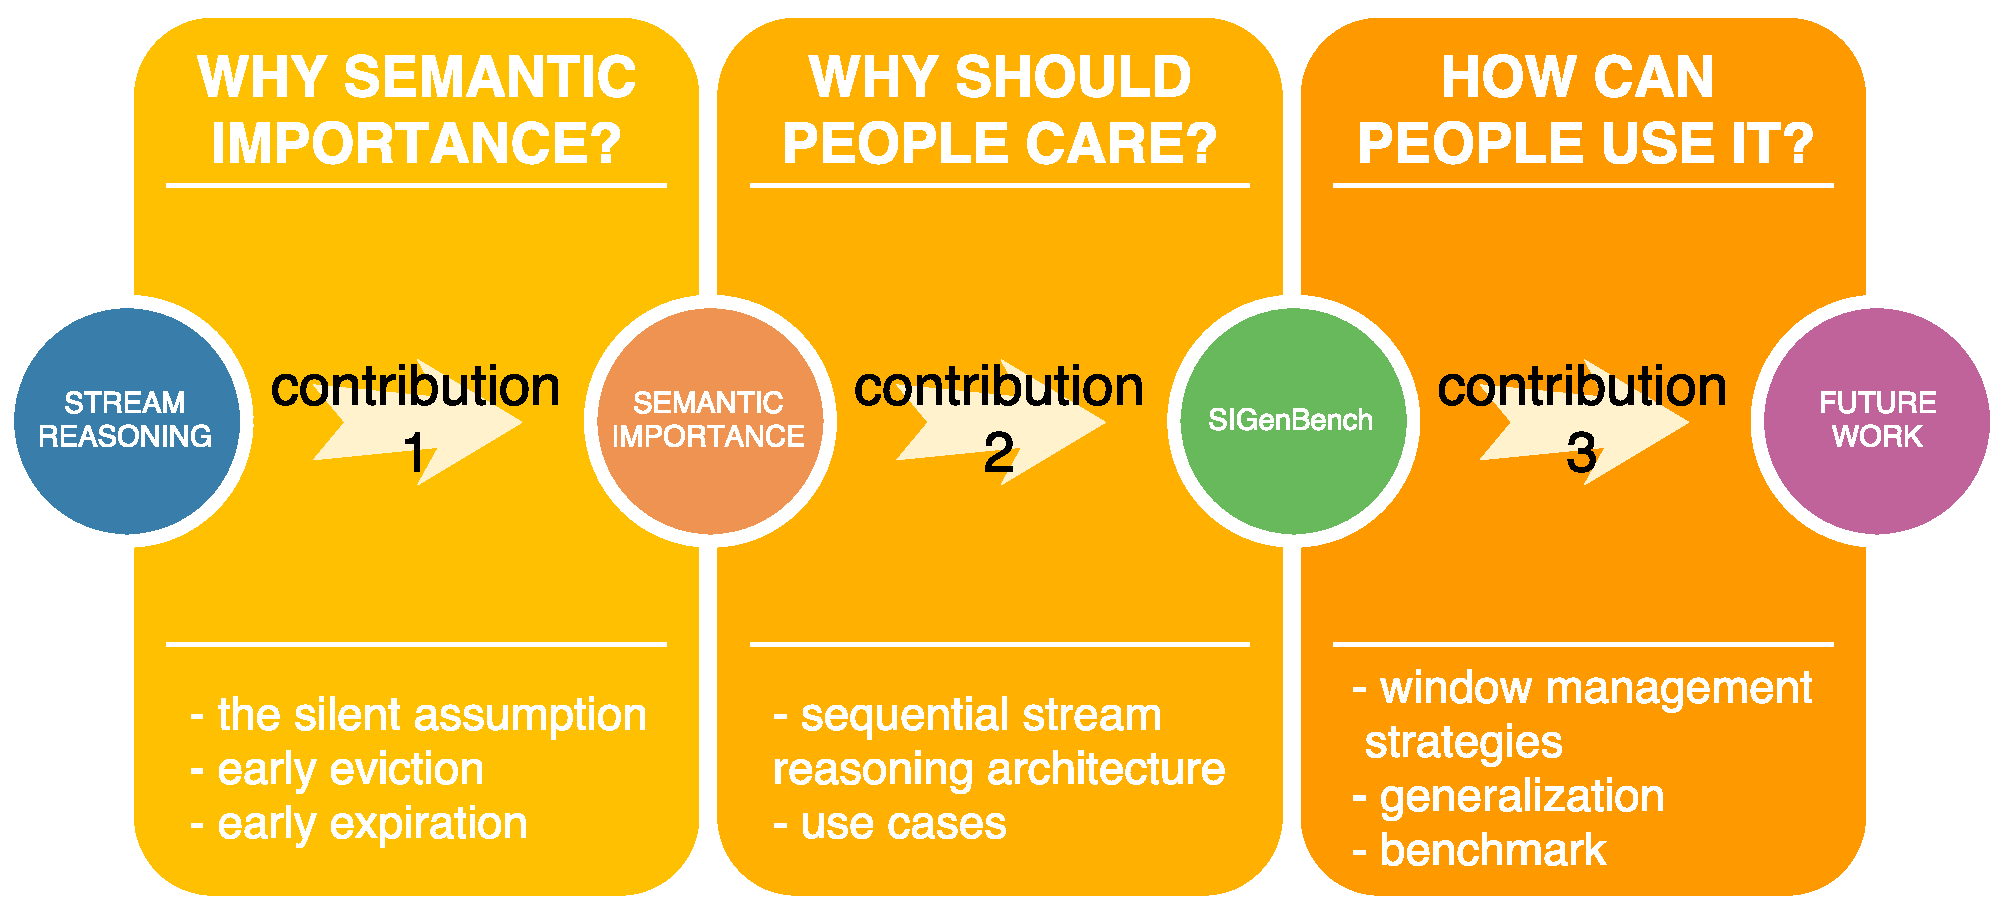
\includegraphics[width=5in]{img/7-trm.pdf}
%     \caption{Thesis Road Map Overview}
%     \label{fig:7-trm}
% \end{figure}
% %
% \subsection{Thesis Brief Review}
% \textcolor{red}{
% Figuhre \ref{fig:7-trm} shows the road map overview of this thesis, which is generally guided by these three questions: 
% ``why semantic importance'', ``why should people case'', and ``how can people use it?''。
% This thesis has rooted itself deeply into the stream reasoning, and targets on smart and flexible streaming data management. 
% }

% \textcolor{red}{
% Chapter 3 covers my first contribution, semantic importance, which is motivated by the observations that the ``silent temporal assumption'' is popular across lots of stream reasoning research work \cite{barbieri2010stream} \cite{stuckenschmidt2010towards} \cite{golab2003processing} \cite{barbieri2010deductive}, and that temporality alone will not work under the situations where the early eviction or expiration problem happens. 
% Semantic importance models the data importance by considering aspects beyond just temporality, such as query participation, query relevance and trustworthiness. 
% It provides a representative schema (priority vector), as well as a set of defined comparison rule to enable data orderings. 
% This answers the first question, ``why semantic importance''.
% }

% \textcolor{red}{
% Chapter 4 introduces sequential stream reasoning architecture (SSRA). 
% It is motivated by the fact that stream reasoning engines such as C-sparql and CQELS are implemented upon the silent temporal assumption, and do not provide an interface to deploy the semantic importance. 
% I have implemented and evaluated SSRA comprehensively.
% Basically I have classified three streaming scenarios and analyzed some of semantic importance enabled strategies' performance. 
% In order to ground both semantic importance and SSRA, I have implemented two use cases in Chapter 5, namely soccer offside detection and data exfiltration detection.
% This thesis has covered detailed implementations and evaluations, and the results show that semantic importance can work under fairly diverse scenarios, as well as provide good precision and response time. 
% However, both of the use cases have some limitations, which I have investigated and explained in this thesis. 
% Thus, the answer to the second question is that, people should care about semantic importance because it can work better than FIFO in the cases where temporality alone is not enough
% It can provide better system performance as well. 
% }

% \textcolor{red}{
% Chapter 6 covers the work to generalize and benchmark semantic importance (SIGenBench).
% Albeit the use case results have indicated that semantic importance is useful, it is not generalized so that a wide range of stream reasoning applications can use it in an easy way.
% SIGenBench connects semantic importance to the state-of-the-art stream reasoning technologies.
% It also comes with a default streaming data generator that simulates different streaming data scenarios. 
% Extensive experiments have been done, and results have been analyzed. 
% SIGenBench answers how people can use semantic importance.
% }
% %
% \subsection{Thesis Wrap-up}
% \textcolor{red}{
% Starting from the Chapter 1, I have been using a running example of the soccer offside detection.
% The purpose of this example is to illustrate the two problems of the streaming data management, i.e. early eviction and early expiration, if temporality is only considered to manage the data.
% }

% \textcolor{red}{
% A window in a stream reasoning application will always evict the oldest data item in order to consume the latest data item, based on the silent temporal assumption, which means that the data is managed by its arrival timestamps: the older it is, the less important it is, thus evicted eventually. 
% However, temporality is certainly not the only criterion to determine the data importance . 
% In the running example, where players' status and positions are so important for the result, the ``who'' (who is attacker or defender?) and ``where'' (where are the players, onside or offside position?) provenance aspects should definitely be considered to manage the data. 
% Thus, my first contribution -- semantic importance is able to provide a multi-dimensional view of the data importance and enable order-aware window management strategies, so that the important data can be captured.
% Examples of the important data include but not limited to: Player A is an attacker, Player A is at the offside position, Player A touches the ball after his teammate passed the ball, etc. 
% Please note that this important data usually does not arrive adjacently, in fact there could be lots of other data arriving in between.
% By keeping the important data, semantic importance can maintain a smaller window size, ideally only to contain the important data items for question-answering, which saves memory and response time.
% Table \ref{tb:accuracy} has already shown that semantic importance enabled strategies (*-LFU-FO, *-LRU-FO, and QR-*) are able to maintain better precision and relatively lower response time than common strategy FIFO, even if the window size shrinks.
% This has already shown the benefits to introduce semantic importance into stream reasoning, and how semantic importance can make the soccer offside offence detection better.
% }

% \textcolor{red}{
% In stead of using C-sparql or CQELS engine to implement the soccer use case, I used my sequential stream reasoning architecture (SSRA).
% This is because I need to enhance streaming data management with semantic importance, which is not supported in C-sparql or CQELS. 
% SSRA is an example of deploying semantic importance in stream reasoning use cases. 
% Its implementation imitates the behavior of other stream reasoning engines.
% The soccer offside detection use case is implemented based on SSRA, and Table \ref{tab:ev} shows all the experimental results.
% SSRA, as my second contribution, shows how semantic importance can be integrated, and performant in real life scenarios. 
% }

% \textcolor{red}{
% My third contribution, SIGenBench, essentially targets on a more general application, including but not limited to the soccer offside detection. 
% The goal is to enable a broad view for semantic importance in the stream reasoning settings. 
% The results from soccer offside use case have already proven that semantic importance can work well. 
% However, more questions need to be addressed, such as how to allow others to leverage semantic importance in their use cases, how to use the mainstream stream reasoning technologies with semantic importance, and under what conditions semantic importance can bring benefits. 
% The answers to these questions are provided by SIGenBench. 
% I have tested four aspects of the current semantic importance, and the results are provided in Table \ref{tab:6-qrp} - \ref{tab:6-fqqi} (query relevance), Table \ref{tab:6-dei} (temporal provenance), Table \ref{tab:6-qpp} (query participation), and Table \ref{tab:6-tp} (trustworthiness). 
% SIGenBench comes with a default streaming data generator that can simulate different streaming data scenarios by configuring parameters such as stream mode and rate. 
% The experiments indicate that trustworthiness and query relevance are both able to tolerate the large and fluctuating data streaming rate, yet query relevance does drop its performance when reaching a relatively large data rate. 
% However, a compound strategy composed by multiple semantic importance aspects such as QR-Trust-FE-LFU-FI-FO is able to provide good performance.
% }
% %
% \subsection{Thesis Key Takeaway Message}
% \textcolor{red}{
% The key message to take away is that, this thesis raises the awareness of the silent temporal assumption, and shows the problems associated. 
% In order to loosen this assumption, this thesis provides a structure -- semantic importance, as well as a set of infrastructure -- SSRA and SIGenBench to use this structure. 
% The experiments results have shown that the smart and flexible window management can be enabled by modeling streaming data importance using semantic importance, as well as that the stream reasoning systems' precision, response time, memory consumption and throughput can be improved.
% }
% %
% \subsection{Thesis Limitations}
% \textcolor{red}{
% Considering that streaming data is huge and can potentially flood the system, the sequential way to process the data clearly has a limit. 
% Parallel processing has lots of benefits, one of them is to boost response time, there are already some examples to leverage distributed systems in stream reasoning \cite{hoeksema2011high} \cite{liu2014efficient}. 
% }

% \textcolor{red}{
% This thesis only deals with RDF streams, which is only a kind of all the streaming data.
% However, in the traffic surveillance scenario, the streaming data is usually video format. 
% This thesis doesn't propose a method for it. 
% }

% \textcolor{red}{
% The query relevance is able to provide good response time and precision, however, as the data rate goes up from Figure \ref{fig:6-csmrrt1} - \ref{fig:6-csmrrt9}, query relevance spends much more time filtering the data and eventually causes a delayed answer. 
% This is a major limitation for query relevance while being used in the sequential processing. 
% However, I presume that this situation will be alleviated in a parallel system. 
% }
% %
% \section{Future Work}
% \textcolor{red}{
% This thesis has covered three contributions for managing the streaming data in the window for stream reasoning applications.
% There are still lots of potential to extend and enhance this work. 
% This section highlights some future work.
% }
% %
% \subsection{Short Term}
% \textcolor{red}{
% This thesis has focused on the temporal provenance, albeit according to \cite{ram2009new}, there are six more aspects including ``what, where, how, who, which, and why''.
% The soccer offside has leveraged where and who provenance, thus this thesis has shown some examples to extend different types of provenance.
% I would like to extend the other aspects of provenance because they provide a broader view and more flexible way to model data importance.
% }

% \textcolor{red}{
% Query relevance is an interesting aspect of semantic importance.
% The experimental results have indicated its effectiveness. 
% For the short term future work, I would like to investigate the general principles to prepare both the query relevance ontology and query relevance filter query. 
% SIGenBench has shown that different query relevance filter queries do have different affects on system performance. 
% If such general principle for preparing query relevance is proposed, the stream reasoning system can be benefited, as well as the users will be benefited from its guidance. 
% }
% %
% \subsection{Middle Term}
% \textcolor{red}{
% SIGenBench is built upon SSRA, which is sequential.
% In the future, I would like to explore some parallel architecture and enhance it with distributed processing systems.
% }

% \textcolor{red}{
% SIGenBench is implemented in Java, which is static typed language.
% All the 26 strategies are implemented as Java classes and hard-coded in the code. 
% If a user wants to use a new strategy, he/she has to dive into my code and add a strategy class manually. 
% There are two planned future work to improve this. 
% First of all, I would like to re-implement SIGenBench by exploiting a dynamic typed language, so that different strategy classes can be generated during the run-time. 
% Secondly, I want to build an ontology loader that can load the semantic importance ontology.
% By combining semantic importance aspect classes, different strategies will be generated proactively. 
% In that way, semantic importance ontology will no longer be a merely descriptive ontology, but actually be used to create strategies.
% }

% \textcolor{red}{
% Long short-term memory (LSTM) \cite{DBLP:journals/neco/HochreiterS97} is a recurrent neural network (RNN), whose cells can ``remember'' values over arbitrary time intervals \footnote{https://en.wikipedia.org/wiki/Long\_short\-term\_memory (Date Last Accessed: Mar. 20, 2018)}.
% LSTM is potentially another way to implement window management strategy, which essentially can capture data items that are arbitrary apart, to alleviate early eviction problem. 
% This is because how much data needs to keep is a similar requirement. 
% I also would like to explore the possibilities to employ LSTM for the streaming data management. 
% }

% \textcolor{red}{
% The default streaming data generator produces fluctuating data based on the observations of the traffic. 
% The future work also includes simulating data bursts based on common burst patterns in other streaming data feeds such as smart city settings \cite{tonjes2014real}.
% }

% \textcolor{red}{
% As we can see from the results in SIGenBench, when data rates increases, some previously working strategies start to fail.
% This can also be found when the data fluctuates a lot.
% I would like to investigate the possibilities to automatically switch strategies in the window so that the data management can be more resilient in different streaming scenarios. 
% }
% %
% \subsection{Long Term}
% \textcolor{red}{
% In this thesis, with only 4 semantic importance aspects, I have created 26 strategies.
% It can be predicted that as the semantic importance ontology is extended, more aspects will create more strategies. 
% Certainly not all of the strategy will help implement the use case. 
% I would like to build a strategy selector in the long time run, with which the users can easily select their desired strategies. 
% In order to realize this, I need to collect data on users' use cases requirements and different strategies performance, which can be done with SIGenBench.
% Then I will use supervised machine learning algorithms to train a model that can recommend strategies for users give their new use case requirements. 
% This future work is dependent upon the general use of semantic importance. 
% }
% \section{Conclusion}
% The core contribution of this dissertation is the notion of semantic importance, along with a set of infrastructure to enable its usage in the stream reasoning settings.
% Exemplar use case implementations have shown show how semantic importance can be leveraged in real-world scenarios.
% The comprehensive generalization and benchmark framework connects semantic importance to the state-of-the-art stream reasoning techniques, which allows testing system performances with multiple dimensional configuration parameters.

% The motivation to propose semantic importance originally comes from the situations where the temporal silent assumption can fail.
% The temporal silent assumption, which regards the most recent data as the most important, only concentrates on one explicit data ordering -- arrival order. 
% This will cause two problems, early eviction and early expiration, as it has been shown in Chapter 1.
% It has been observed that these two problems are caused because the system is not able to distinguish the data based on its priority. 
% Such priority, often implicit, leads to the efforts to make it visible for the processing system, which is formalized in the concept of semantic importance.
% Semantic importance is derived from various data orderings, and currently provides four general aspects that can support a wide range of window management strategies.
% Like FIFO, these strategies help window to identify more important data with one or multiple data orderings; but unlike FIFO, these strategies provide more flexible options to choose under different stream reasoning scenarios, which can improve system performance.

% Chapter 3 shows what semantic importance is, as well as its incompatibility with the existing window semantics that only works with FIFO.
% In order to deploy semantic importance in stream reasoning systems without breaking the integrity of window semantics, the landmark window is leveraged.

% The semantics of landmark window provide a firm theoretical foundation for the application of semantic importance. 
% Stream reasoning not only requires real-time stream processing, but also on-line reasoning.
% Most state-of-the-art work in stream reasoning performs logical reasoning, i.e., to provide a background ontology that contains the knowledge about the domain in the window.
% A reasoner also resides in the window, which can be used to infer hidden information together with the ontology and the streaming data. 
% However, logical reasoning is relatively slow, and does not scale well with large volume of data. 
% One method to minimize this problem is to reduce the data items in the window. 
% This can be done by either shrinking the window size or filtering the data. 
% When shrinking the window size, data items get more easily to exit the window under the silent assumption, but when filtering data, the system has to make sure to filter data correctly so that all the necessary data items are kept. 
% Both of them require the system to be data discriminative, which is enabled by semantic importance. 

% Semantic importance currently includes four aspects, provenance, query participation, trustworthiness, and query relevance. 
% It is designed to be flexible and extendable. 
% It also comes along with an ontology that is grounded by real-life use case and instances.
% Semantic importance is embodied in a priority vector, which features a preference function that the most preferred element is placed leftist, as well as a comparison rule that enables ranking.

% The semantics of sliding window, which works well with the temporal silent assumption, cannot be adopted when using semantic importance. 
% This is because, other than FIFO, the strategies enabled by semantic importance will evict the data out of its arrival order.
% This can break the semantics of the sliding window.
% Thus, the landmark window is proposed to use, as its semantics works well under the semantic importance framework. 
% Both time-based and tuple-based window semantics have been refined, which is not only compatible with the sliding window, but also opens up more window options to use in stream reasoning. 

% Chapter 4 introduces the sequential stream reasoning architecture (SSRA), with the purpose of providing the first architecture to deploy semantic importance for stream reasoning use cases. 
% SSRA features five main component, other than the window implemented in off-the-shelf triple-stores, the data consumption component consumes the data by sending it into the window. 
% Depending on different window report policies, the query execution component is fired and thus query results are generated. 
% The reasoner inside of the triple-store can provide the ability to trace back to what happened during the reasoning and query process, such that the data items participated in the query can be tracked.
% At last, the data is evicted based on its semantic importance ranking.
% Usually, the lower-ranked data will be evicted first. 

% SSRA shows how semantic importance can be deployed in a stream reasoning application, with experimental evidence that shows SI efficacy. 
% Since most state-of-the-art stream reasoning work is dependent on solely sliding window, which encapsulates the window and window strategies within the internal core, it is not feasible to implement semantic importance on the top of them. 
% However, their architecture and design can be referenced, which leads to the sequential stream reasoning architecture. 
% The core design is to let the window stand out of the processing architecture, so that it can be configured according to the users' need. 


% Chapter 5 shows two use cases implementations based on different window management strategies.
% Both of them are within the streaming context, where the data is either streamed in high frequency or large volume. 
% They are real-world use cases with different requirements.
% The results have shown that semantic importance is adaptable in different cases, and provide satisfactory system performance. 

% Chapter 6 generalizes semantic importance by connecting it to the state-of-the-art stream reasoning techniques, as well as provides a software that can benchmark the performance of stream reasoning applications.
% The experimental results have provided a systematical analysis on how different factors can affect the system performance, as well as how semantic importance can help minimize the adverse impacts and maximize the benefits. 
% SIGenBench is carefully implemented to decouple the window semantics out of its processing engine, such as C-sparql and CQELS. 
% Currently, SIGenBench supports four kinds of window, four kinds of window report operational semantics, two kinds of continuous query language, and twenty-four different window management strategies. 
% All of these open up a greater possibility to configure windows in many different ways. 
% SIGenBench can also control stream rates and modes, so as to provide more simulation capabilities. 
%
% \section{Future Work}
% Semantic importance currently only has four aspects, among which the provenance and trustworthiness aspects are both very broad. 
% This dissertation only talks about some temporal provenance, and leaves other types of provenance untouched. 
% For example, geographical location is an example of non-temporal provenance, and surely can be useful for some queries that involve geology.
% Query relevance is a very interesting aspect. 
% There are several ways to make it more interesting in the future.
% For example, formalize the general principles of preparing the query relevance ontology, although in Section 3.4 I have briefly mentioned this. 
% Since query relevance ontology is static and will only work with one query. 
% This hinders system if a different query is deployed. 
% Another direction is to come with a method to enable query relevance self-evolving ontology.
% Basically it can learn what is going on in the current stream and summarize some potential interesting knowledge. 
% From the experiments, it has also shown that different query relevance filtering queries have different impacts on system performances. 
% The next step also includes how to come up with good filter queries that maximize the performance gain, to formalize the criterion for categorizing and recognizing good, OK or bad queries.
% One future work is to explore and expand semantic importance both horizontally and vertically.

% SIGenBench is a tool that helps test semantic importance.
% It is configured with parameters in the command lines. 
% Users can feed their data, ontology, and choose their desired window and stream configurations before any experiments can run, from which the benchmark results will be generated.
% One restriction in this tool is that, all the strategies are currently built-in, which does not enable the user to choose their own desired strategies that are not listed within. 
% The reason is because SIGenBench is implemented in Java, which is a static type language, and does not support explicitly creating undeclared classes during the run-time. 
% There is really no solution to this in Java, thus what I did was to hard code all 26 strategies in the explicit class files and call them during the run time.
% There are two directions in the future work to enhance it.
% First, to implement SIGenBench in a dynamic typed language, so that the strategies can be created during the run-time.
% Second, the strategies will be supported by loading the semantic importance ontology, where the users extend, specify and edit their extended aspects.
% SIGenBench should be able to create a list of possible strategies on the top of reading semantic importance ontology and let the user to specify what strategy they would like to test in their use cases. 

% The third future work is a more ambitious one.
% As time goes by, during which semantic importance is being used and extended, as well as different use cases are being developed, the data of both use case requirements, the chosen management strategies and semantic importance aspects will become more and more available quantitatively and in quality.
% By leveraging such data and supervised machine learning algorithms, a recommendation system should be feasible to implement, and able to provide some constructive suggestions on which semantic importance aspects and strategies to use for new users, based on the input of their use cases. 
% The recommended results will be at least as a starting point from which the users will need to test their use case. 